\documentclass[aps,pre,twocolumn,superscriptaddress,showpacs]{revtex4-1}
%
%==================================================================
% PREFACE
%==================================================================
%
% BibTeX
\bibliographystyle{apsrev}
\bibliographystyle{plain}
%
%Packages
\usepackage{natbib}
\usepackage[english]{babel}
\usepackage[dvips]{graphics}
\usepackage{graphicx,epsfig}
\usepackage{amsmath}
\usepackage{color}
\usepackage{float}
\usepackage{multirow}
\usepackage[normalem]{ulem}
\usepackage{booktabs}
\usepackage{amsfonts} 
\usepackage{multirow}
\usepackage{subcaption}
\usepackage{braket}
\usepackage{caption}
\captionsetup{justification   = raggedright,
              singlelinecheck = false}

%\allowdisplaybreaks

\newcommand{\om}{\omega}
\newcommand{\omx}{\omega_1}
\newcommand{\omy}{\omega_2}
\newcommand{\En}{\mathcal{E}_n}
\newcommand{\abinitio}{\textit{ab initio }}

%Text commands
\newcommand{\CR}[1]{{\color{red}{#1}}}
\newcommand{\CB}[1]{{\color{blue}{#1}}}
\newcommand{\CG}[1]{{\color{green}{#1}}}
\newcommand{\no}[1]{{\sout{\color{red}{#1}}}}
\newcommand{\nob}[1]{{\sout{\color{blue}{#1}}}}
\newcommand{\bfeq}[1]{{\boldsymbol{#1}}}

\begin{document}
\title{Improving Inelastic Confinement-Induced Resonances calculations on the CRC model}
%
\author{T. Sanchez-Pastor}
\affiliation{Grupo de Sistemas Complejos,
Escuela T\'ecnica Superior de Ingenier\'ia Agron\'omica,
Alimentaria y de Biosistemas,
Universidad Polit\'ecnica de Madrid,
Avda. Puerta de Hierro 2-4, 28040 Madrid, Spain.}

\author{Alejandro Saenz}
\affiliation{AG Moderne Optik, 
Institut für Physik, 
Humboldt-Universität zu Berlin, 
Newtonstrasse 15, 12489 Berlin, Germany.}

\author{F. Revuelta}
\affiliation{Grupo de Sistemas Complejos,
Escuela T\'ecnica Superior de Ingenier\'ia Agron\'omica,
Alimentaria y de Biosistemas,
Universidad Polit\'ecnica de Madrid,
Avda. Puerta de Hierro 2-4, 28040 Madrid, Spain.}
%
%------------------------------------------------------------------------------------
\begin{abstract}
In this work we study several aspects of the Inelastic Confinement-Induced Resonances caused by the coupling of center-of-mass and relative motion for a system of two Lithium ultracold atoms in anharmonic sextic traps. We take advantage of the \abinitio calculations to ensure the CRC model robustness presented in [Phys. Rev. Lett. \textbf{109} 073201 (2012)] computing the exact trap relative motion energy of the resonance. We generalize the theoretical resonance position as a function of a parameter $\mathcal{C}$ and give exact results of the theory predictions for a wide range of this parameter in 3-D and quasi 1-D optical traps. Shadow bands corresponding to the predictive limit of the theory are also presented. Within the theoretical results we also study the main differences between both confinements. Finally, we build a perturbative model in order to describe in depth the origin of the asymmetric splitting of the resonances.
\end{abstract}
%------------------------------------------------------------------------------------
%\pacs{05.45.-a, 33.20.Tp, 82.20.-w}

\maketitle

%------------------------------------------------------------------------------------
\section{Introduction}  \label{sec:intro}
Contar un poco de historia de la observación de este tipo de resonancias, por qué los sistemas ultrafríos están de moda (control) y resonancias de 	Feshbach (cambiar B es cambiar a). 
Acoplamiento CM-rm como causante de los cruces evitados, transiciones no adiabáticas y rmacionarlo con el teorema adiabático.
%------------------------------------------------------------------------------------
\section{Two-atom numerical simulations}  \label{sec:system}
In this section we present the Hamiltonian that describes the interaction between two ultracold-atoms trapped in anisotropic optical lattices (Sec.\ref{subsec:H}). Also, ab initio calculations to 
simulate the system is presented in Sec.\ref{subsec:Ab_initio}.

\subsection{Hamiltonian} \label{subsec:H}
The system is formed by two Lithium ultracold atoms that interact only via s-wave scattering due to the extremely low temperature of the gas. The last leads to a spatial symmetry where
rm andCM coordinates reduce the complexity of the calculations. Relative motion distance is defined as $\bfeq{r} = \bfeq{r_1} - \bfeq{r_2}$ whereas CM coordinate as 
$\bfeq{R} = \frac{1}{2}(\bfeq{R_1} + \bfeq{R_2})$. The Hamiltonian is then given by:
		
\begin{eqnarray}
\mathcal{H}(\bfeq{r}, \bfeq{R}) &=& T_{CM}(\bfeq{R}) + T_{rm}(\bfeq{r}) + V_{CM}(\bfeq{R}) +  \nonumber \\ 
&+& V_{rm}(\bfeq{r}) + W(\bfeq{r}, \bfeq{R}) + U_{int}(|\bfeq{r}|), 
 \label{eq:Hamiltonian}
\end{eqnarray}
		
where the $T$'s are the kinetic energy operators and the $V$'s the separable potential energies for both rm and CM coordinates, while $W$ accounts for the rm-CM coupling, which is 
nonzero for anharmonic traps. The coupling term is responsible of 	the avoided crossings and therefore of the ICIR. $U_{int}$ is the particle-particle potential energy often 
described in analytic derivations by the pseudopotential $U_{int} = \frac{4\pi \hbar^2 a_s}{m} \delta(\bfeq{r})\frac{\partial}{\partial \bfeq{r}}$, where $a_s$ is the 3-D s-wave scattering length.
		
In a 3-dimensional optical trap the potential terms are
\begin{eqnarray}
V_{rm}(\bfeq{r}) &=& 2 \sum_{j=x,y,z} V_j \sin^2 \left(\frac{1}{2}k r_j \right), \\
V_{CM}(\bfeq{R}) &=& 2 \sum_{j=x,y,z} V_j \sin^2 \left(k R_j \right), \\
W(\bfeq{r}, \bfeq{R}) &=& -4 \sum_{j=x,y,z} V_j \sin^2 \left(\frac{1}{2}k r_j \right) \sin^2 \left(k R_j \right).
\end{eqnarray}
		
$k$ is the angular wavenumber and $V_j$ the potential depth in any direction. Associated with the potential depth, the trap frequencies are $\omega_j = k\sqrt{\frac{2V_j}{m}}$ and the
 characteristic trap length $d_j = \sqrt{\frac{2\hbar}{m\omega_j}}$. Thus, the anisotropies can be defined in units of the transversal component: $\eta_j = \frac{\omega_j}{\omega_y}$.
	
	
\subsection{Ab Initio calculations} \label{subsec:Ab_initio}
Schrödinger equation is solved using the full six-dimensional Hamiltonian of eq.(\ref{eq:Hamiltonian}) in spherical coordinates. The exact 	diagonalization is carried using realistic 
short-range interatomic potentials: numerically Born-Oppenheimer curves. The interaction potential is then varied to tune the scattering length. Regarding the trap potential we 
expand to sixth order to account for anisotropies associated with non-vanishing coupling terms.  We use a basis set of B-splines and spherical harmonics for the angular dependencies.
\cite{PhysRevA.84.062710}
		
The computation of the eigenenergies and eigenfunctions is obtained in a two-step method as follows: (i) First, the separable part of the Hamiltonian is diagonalized in order to compute
the eingenfunctions $\ket{\psi^{rm}_n}$ and $\ket{\Psi^{CM}_{\bfeq{m}}}$, which will be called \textit{orbitals} because of their similarity to the electronic orbitals used in Quantum Chemistry.
(ii) The coupling remaining term is solved building a new basis. The states of this basis are the so-called \textit{configurations} $\ket{\Phi_{n, \bfeq{m}}} = \ket{\psi^{rm}_n \Psi^{CM}_{\bfeq{m}}}$.  
		
Ab initio calculations are used to compute the dependence of the eigenenergies on the scattering length for a wide range of anisotropies $\eta_x$. The center points of the avoided crossings 
are the positions of the ICIR that we compare with the theory predictions.
%------------------------------------------------------------------------------------
\section{Improving ICIR calculations}  \label{sec:theory}
This section is devoted to dig into the CRC model used in other works to predict the ICIR positions. First, we explain its main assumptions, limitations of the model and we propose a
method to compare ab initio and model predictions. In Sec. \ref{subsec:3D} we present the results for a 3-D trap: the complete dependence of the spectrum on the scattering length $a_s$ and
the resonance positions for numerous anisotropies. Finally, we present similar results for a quasi 1-D trap in Sec. \ref{subsec:quasi 1-D}.
	
In order to locate the resonance in the energy spectrum, exact solutions of the anharmonic traps are needed. However, an exact solution remains unknown yet. In contrast to this, an exact solution
has recently been developed for fully anisotropic harmonic confinements in \cite{PhysRevA.101.053624} and in \cite{PhysRevA.102.013314}, where the solutions of \cite{PhysRevA.74.022712} and
 \cite{Liang_2008} have been generalized. 
	
ICIR have its origin in the avoided crossings between the relative least bound state with CM excitations $\ket{\psi^{(b)}(\bfeq{r}) \Psi_{\bfeq{n}} (\bfeq{R})}$ and the lowest trap state
$\ket{\psi^{(1)}(\bfeq{r}) \Psi_{(0,0,0)} (\bfeq{R})}$ (next excited states of the trap are empty due to low thermal energies).  Thus, the crossings satisfy the relation: $E_b = E_1$, where the 
bound state energy is $E_b = E^{rm}_b + E^{CM}_{\bfeq{n}}$ and the trap state energy $E_1 = E^{rm}_1 + E^{CM}_{(0,0,0)}$. Theory provides an analytic expression to implicitly relate the
bound relative energy with the scattering length as follows:
\begin{eqnarray}
\frac{\sqrt{\pi} d_y}{a_s} &=& \nonumber \\
 - \int^\infty_0 &dt& \left( \frac{\sqrt{\eta_x \eta_z} e^{\frac{\epsilon t}{2}}}{\sqrt{(1 - e^{-t}) (1 - e^{-\eta_x t}) (1 - e^{-\eta_z t})} } - t^{-\frac{3}{2}}\right). \nonumber \\
\label{eq:ascE}
\end{eqnarray}
	
$\epsilon = \frac{E^{rm}_b - E_0}{\hbar \omega_y}$ is the energy shift and $E_0 = \frac{\hbar}{2}\sum_j \omega_j $ the ground state energy of the CM for a harmonic trap. Using the above
expressions the energy shift can be described by:
\begin{equation}
\epsilon = \frac{E^{rm}_1 - E^{CM}_{\bfeq{n}} + E^{CM}_0 - E_0}{\hbar \omega_y}
\label{eq:Energy shift}
\end{equation}
	
The two cornerstones of the CRC model are: (i) assume the anharmonicities are small enough to be treated as perturbations. (ii) The ICIR occurs when the eigenenergy $E^{rm}_1$
of the first trap state $\ket{\psi^{(1)}}$, which lies in the interval $[E_0, E_0 + 2\hbar \omega_z)$, is $E^{rm}_1 = E_0 + \hbar \omega_z$ \cite{PhysRevLett.109.073201}. In this work, we study 
the validity of the second assumption considering the ICIR to happen at
\begin{equation}
E^{rm}_1 = E_0 + \mathcal{C} \hbar \omega_z,
\label{eq:C equation}
\end{equation}
	
where $\mathcal{C} \in [0, 2)$ is a parameter to determine using the ab initio ICIR positions. As will be later demonstrated, in the case of quasi 1-D traps, the assumption of $\mathcal{C}=1$
works relatively fine, but when more CM excitations are present or the trap is not excessively anisotropic, a smaller value of $\mathcal{C}$ is more accurate. Therefore, subsituying Eq. \ref{eq:C equation} into Eq. \ref{eq:Energy shift}

\begin{equation}
\epsilon = C\eta_z - \frac{E^{CM}_{\bfeq{n}} - 2E^{CM}_0 + E_0}{\hbar \omega_y}
\label{eq:final energy shift}
\end{equation}
	
Recall that $\mathcal{C} \hbar \omega_z$ gives the energy difference between the resonance energy and the asymptotic energy $E_{\infty}$ of the first excited state for $\frac{d_y}{a_s} \to \infty$
(limit of noninteracting particles). Then, the $\mathcal{C}$ parameter can be computed as
\begin{equation}
\mathcal{C} = \frac{E_{ICIR} - E_{\infty}}{\hbar \omega_z}.
\end{equation}
	
In this manner, this approach accounts for trap anharmonicities since $E_{\infty}$ is chosen the energy of the asymptotic configuration. Furthermore, the energy of the resonance $E_{ICIR}$ is 
obtained with ab initio calculations, which means that also takes into account the coupling terms.    

\subsection{3-D} \label{subsec:3D}
We start the calculations in the totally symmetric trap, where the eigenenergies are degenerated in the three spatial directions. As said, the scattering length is tuned while changing the Born-Oppenheimer potential. Thus, the fully coupled-adiabatic spectrum is shown in Fig.\ref{fig:q3d ICIR}.a). The CM excited bound states can be easily identified due to they tend to zero when the scattering length also tends to zero. The lowest curve corresponds with the ground state $\ket{ \psi^{(b)} \Phi_{(0,0,0)} }$ and the next three degenerated states with two CM excited bound states. Close to them we found the first trap state $\ket{ \psi^{(1)} \Phi_{(0,0,0)}} $ that only causes resonances for repulsive potentials ($a_s > 0$). 

The width of the avoided crossings is proportional to the coupling strength, therefore the existence of resonances is governed by the laser intensities. A key feature of the 3-D case is that all spatial directions can contain resonances. Unfortunately, the resonances of $\ket{ \psi^{(b)} \Phi_{(2,0,0)}} $ and $\ket{ \psi^{(b)} \Phi_{(0,2,0)}}$ are not found to every value of the anisotropy $\eta_x$ as for the quasi 1-D case, despite of that we study the resonances  $\ket{ \psi^{(b)} \Phi_{(4,0,0)}} $ and $\ket{ \psi^{(b)} \Phi_{(0,4,0)}}$.
\begin{figure*}[htbp!]
\centering
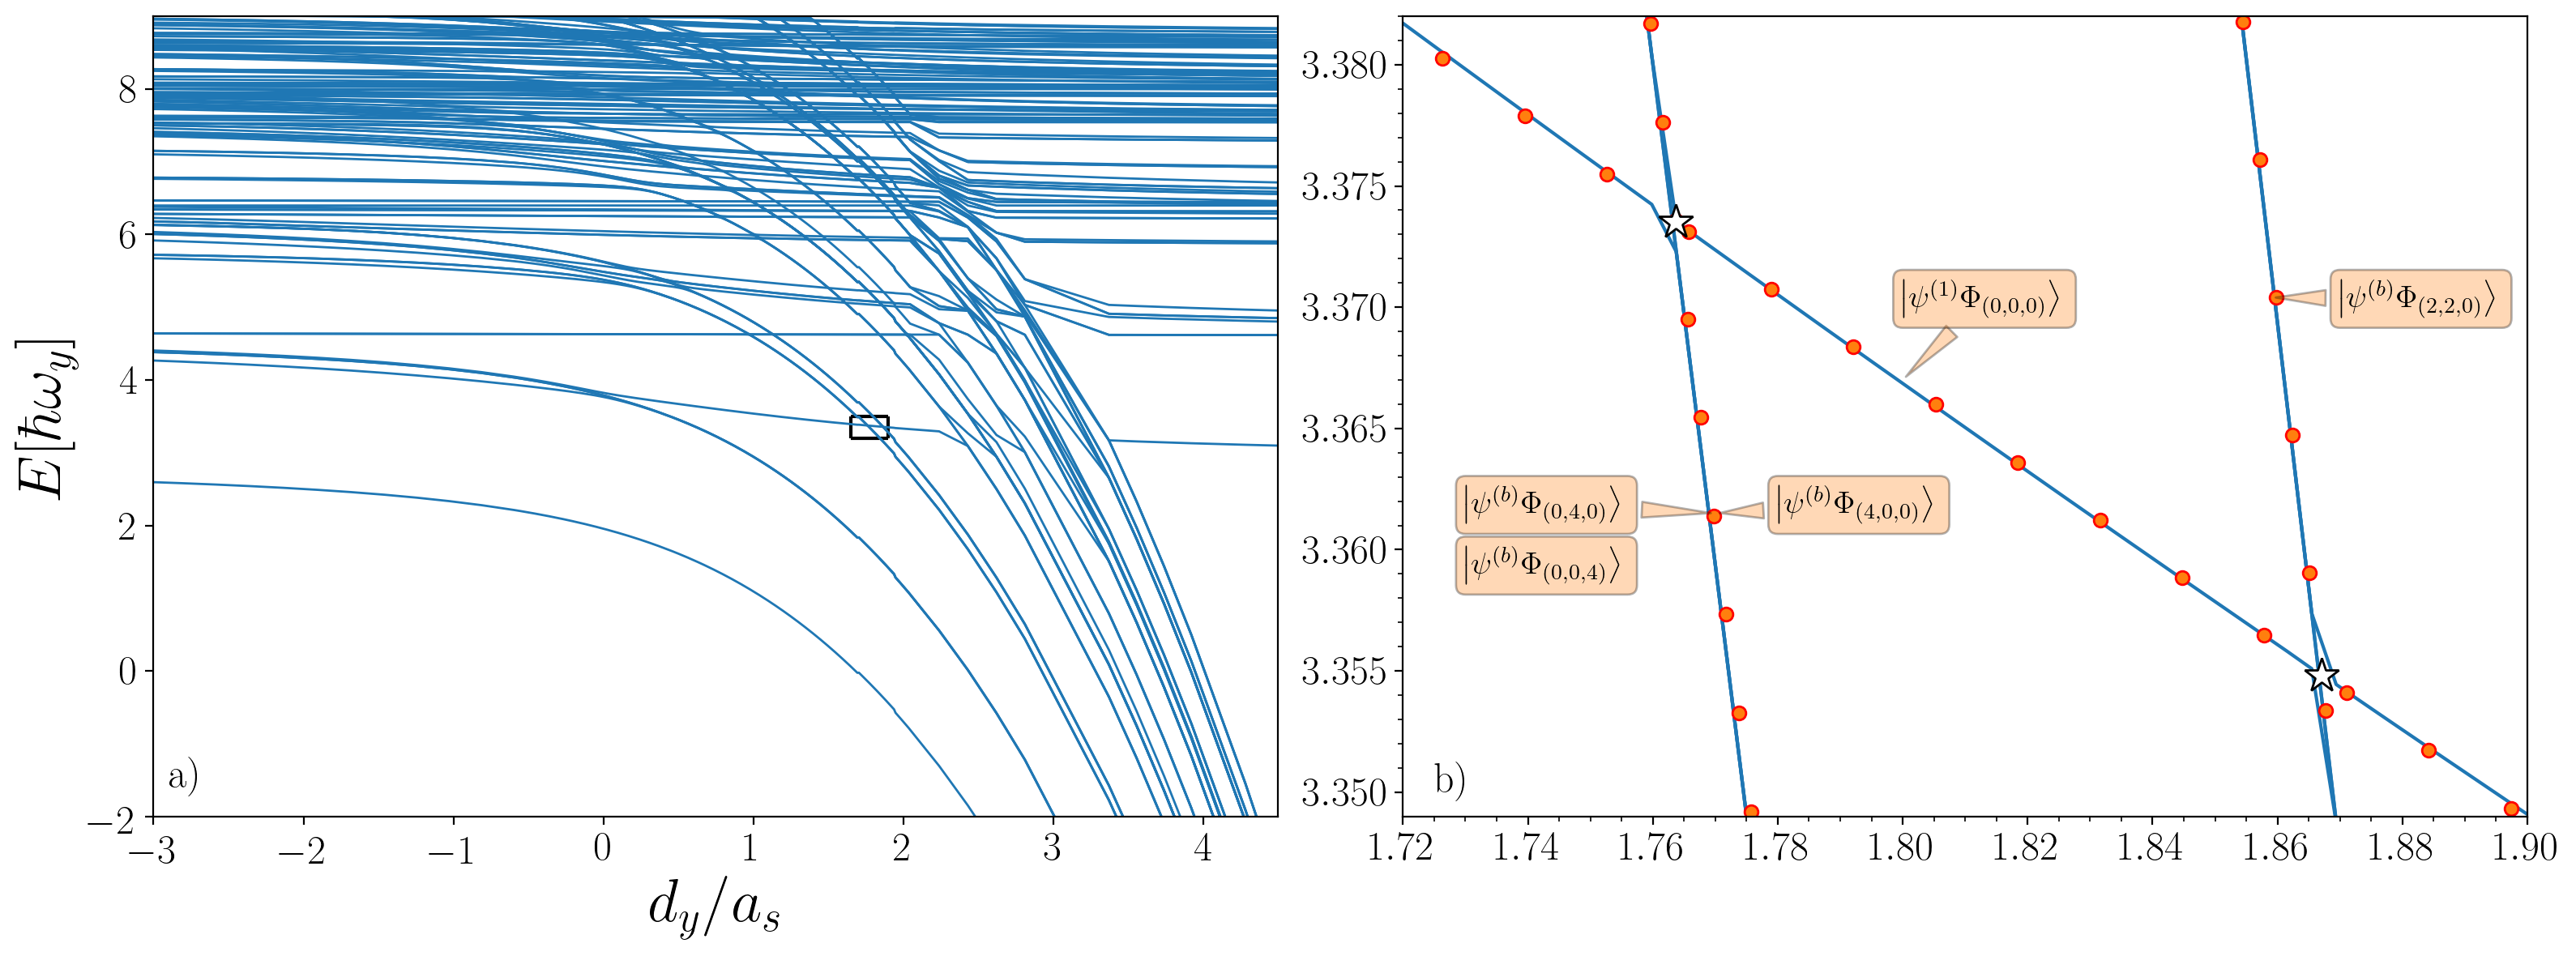
\includegraphics[width=\textwidth]{/Users/tomy/PhD/Ultracold_Atoms_src/Analysis/q3d/Results/Figures/Ix4993_Iy4993_Iz4993_Spectrum_Zoom.png}
\caption{a) Adiabatic Spectrum of the full coupled Hamiltonian for $^7$Li atoms confined in an isotropic sextic trapping potential with $V_x = V_y = V_z = 35.9E_R$, $\eta_x = \eta_y = 1$ and 
$\lambda=1000$ nm where $E_R = \frac{\hbar^2k^2}{2m}$ is the photon recoil energy. All states bending down to $-\infty$ are molecular states originating from the rm bound state $\psi^{(b)}$ 
with different CM excitations, whereas the states remaining constant are trap states of different rm excitations $\psi^{(1)}$ and zero CM excitations. Black square zoom in figure b) where diabatic 
levels are plotted with orange circles and labeled by kets. White stars represent the cross between trap and bound CM excited states, i.e. the ICIR.}
\label{fig:3D spectrum}
\end{figure*}

In Fig. \ref{fig:3D spectrum}. b) the adiabatic and diabatic energies are represented, as well as de ICIR positions. The effect of increasing the longitudinal anisotropy on the spectrum resides in a breaking of symmetry of the trap. The energy degeneracy is also broken and the isotropic resonance splits in two.

Repeating the same calculations for longitudinal anisotropies $\eta_x$ from $1$ to $1.25$  leads to a wide range of ICIR positions.  These positions will be further used to computing the $\mathcal{C}$ parameter with the Eq.\eqref{eq:C equation} and thus validate the CRC model. Each resonance has four predictions associated with it depending on the value of the parameter: exact $\mathcal{C}$ arising from the exact ICIR position, $\mathcal{C} = 1$ corresponding to the assumption of previous works, the lower limit $\mathcal{C} = 0$ and the upper limit $\mathcal{C}=2$. Limit values serve to constrain the predictions of the theory, they will be represented by shadow bands where each of the four previous predictions will fall within them. With regard to the excitation energies of the CM, they have been calculated numerically using a sinc-DVR method.

\begin{figure}[htbp!]
 \centering
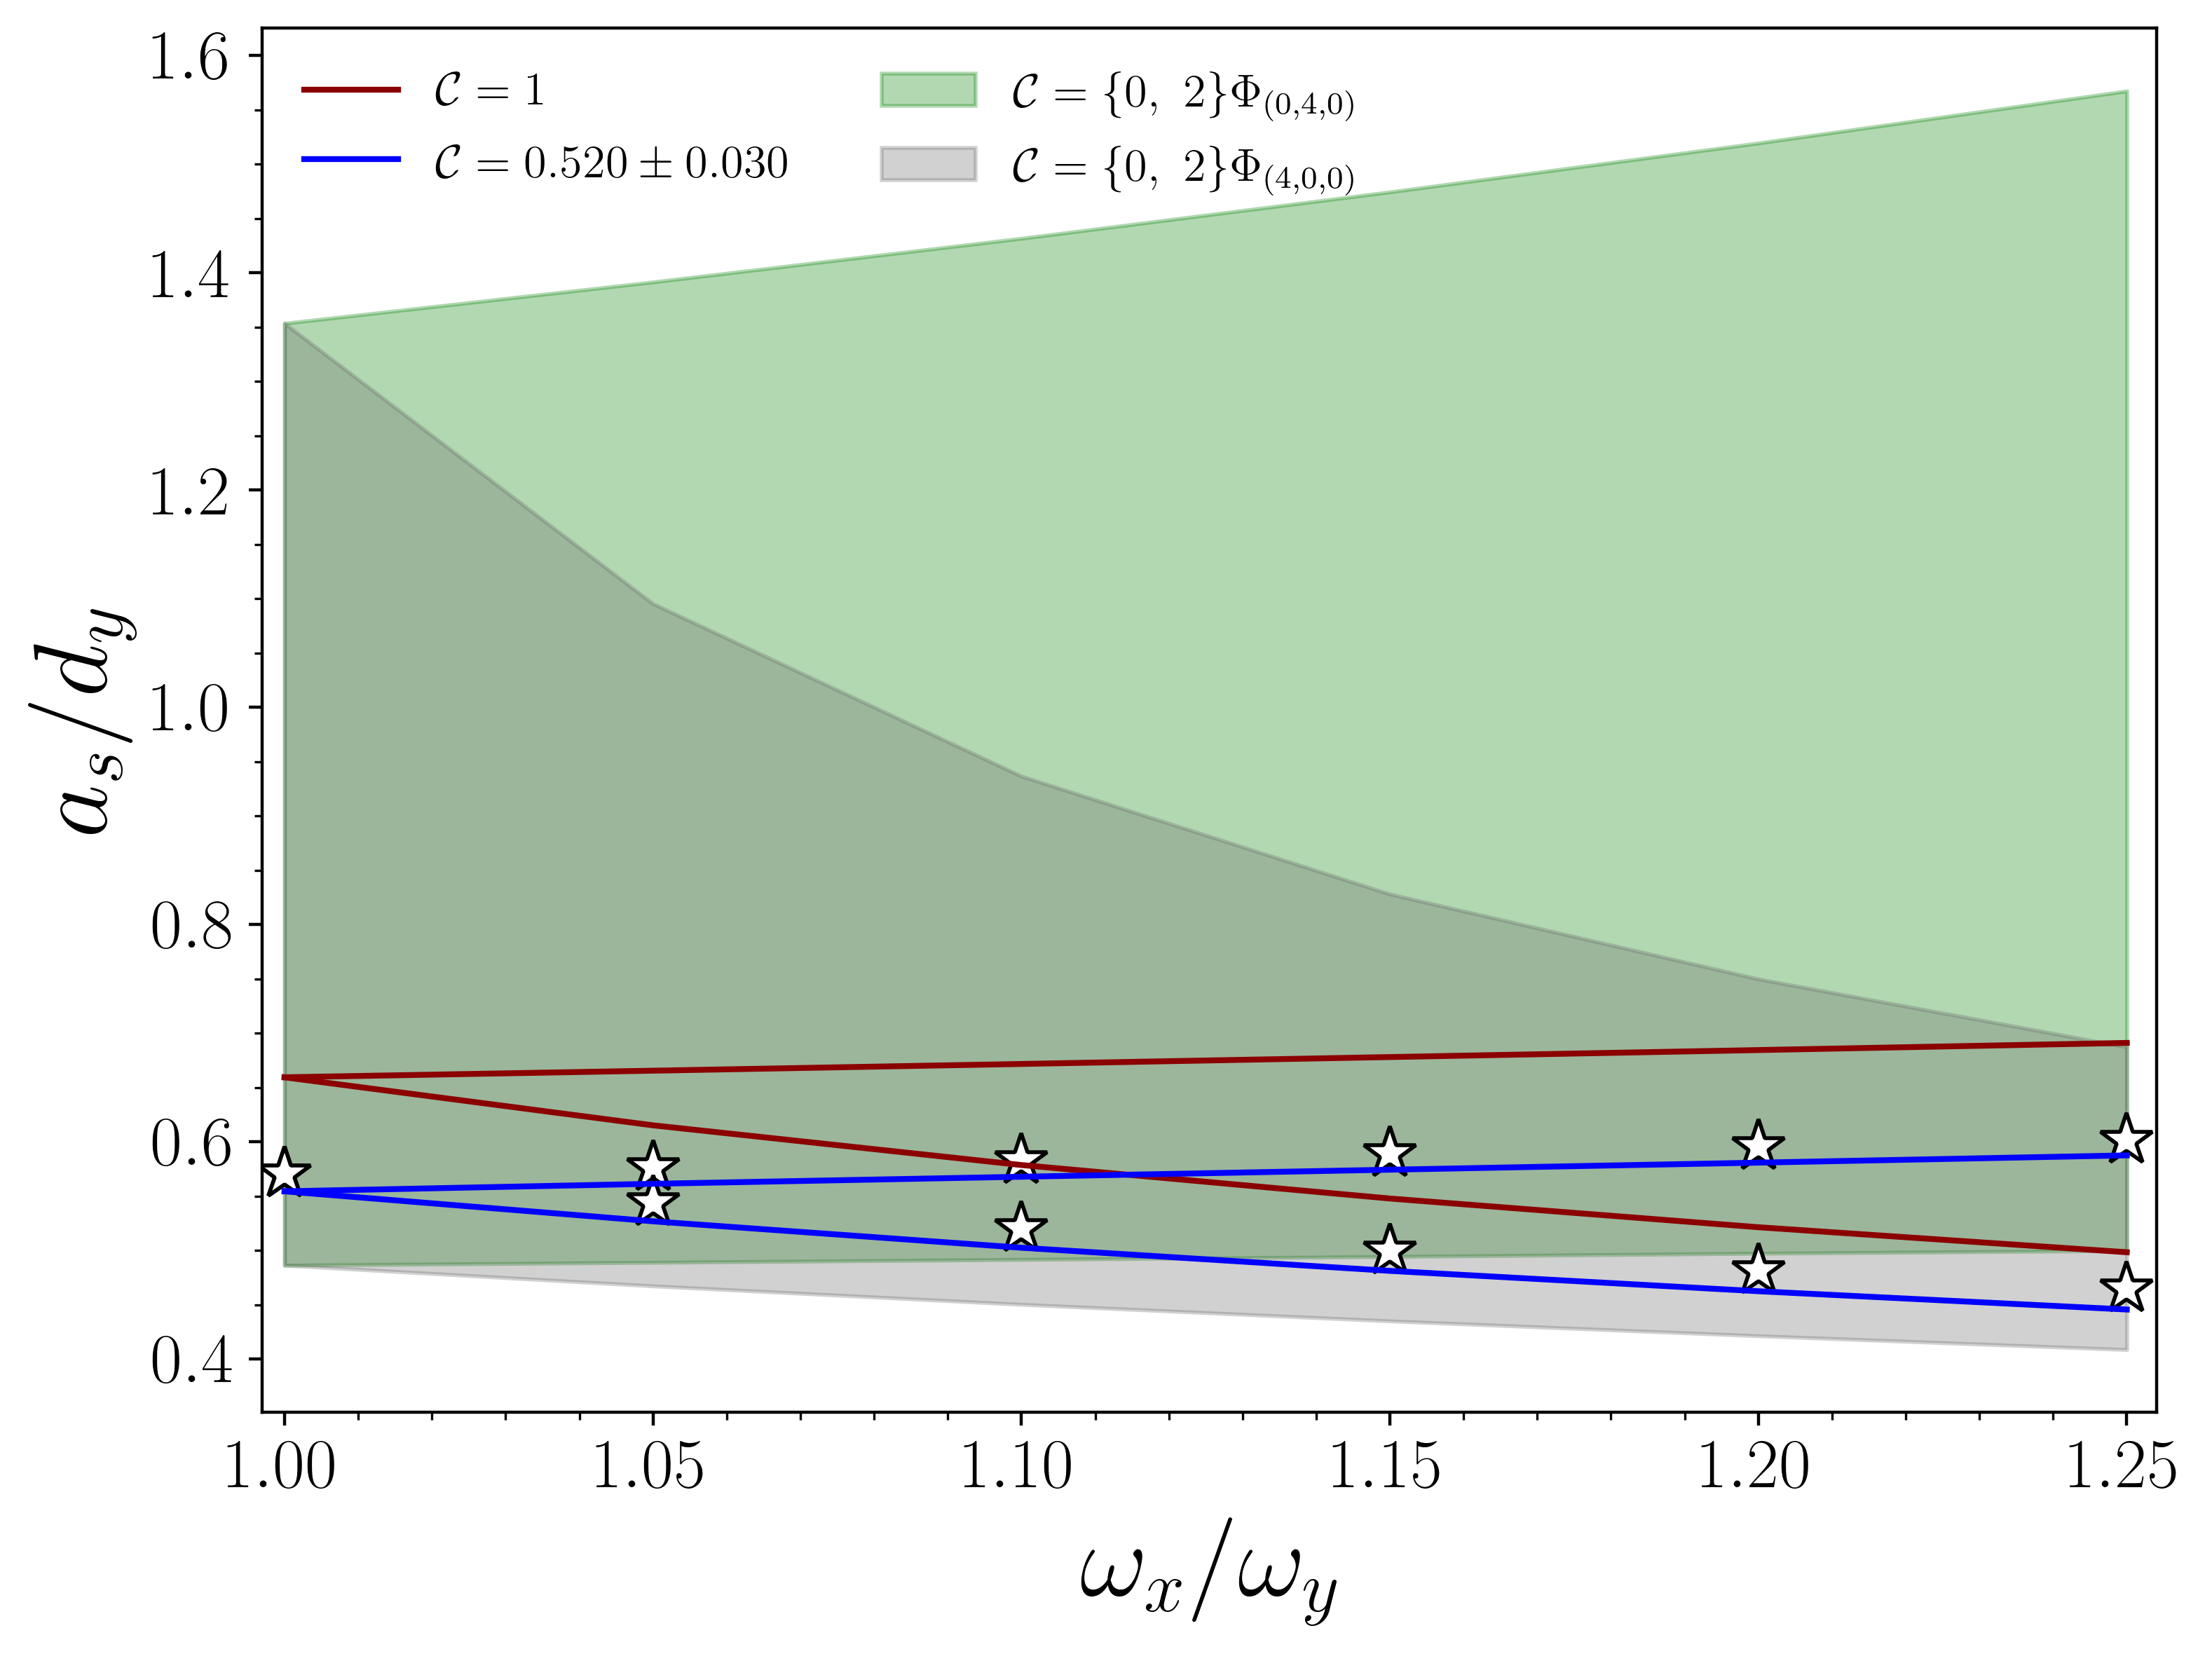
\includegraphics[width=0.5\textwidth]{/Users/tomy/PhD/Ultracold_Atoms_src/Analysis/q3d/Results/Figures/ICIR_q3D_Theory_band.png}
 \caption{Positions of the ICIR associated with four CM excitations in terms of the characteristic transversal length for different values of transversal anisotropy in 3-D. White stars become from ab initio calculations, blue solid lines the exact theory computations, red solid lines $\mathcal{C}=1$, gray shadows the corresponding theory computations with both $C=2$ and $C=0$ for the longitudinal resonances and green shadows for the transversal resonances. }
 \label{fig:q3d ICIR}
 \end{figure}

Figure \ref{fig:q3d ICIR} contains the ICIR's position as a function of the longitudinal anisotropy $\eta_x$ of the \textit{ab initio} calculations and the modified CRC model. The mean value and the deviation of the set of exact $\mathcal{C}$ obtained for all the resonances are $\mathcal{C} = 0.52 \pm 0.03$. In addition, the mean absolute error (MAE) between the prediction and the \textit{ab initio} calculations is $1.6 \cdot 10^{-2}$. On the other hand, the MAE obtained using $\mathcal{C} = 1$ is $7.3 \cdot 10^{-2}$, four times greater than for the exact $\mathcal{C}$.  The origin of this discrepancy between the second CRC model assumption and our calculations is more pronounced in the 3-D case, as a result of the extreme level mixing characteristic to this confinement dimension that displaces the diabatic crossings from the isotropic harmonic case. We will further discuss this result in Sec. \ref{subsec:quasi 1-D}.  Concerning the shadow bands, it is interesting the fact that $\mathcal{C} = 0$ achieve better results than $\mathcal{C}=2$ for every anisotropy and it is ununderstandable without a proper perturbative approach. In the same line, asymmetric splittings of the ICIR between the limit values are explained within perturbative schemes in Sec. \ref{sec:perturbation}. 
		 
We have verified that using \textit{ab initio} calculations to compute the ICIR position is necessary in 3D confinements; on the one hand the exact $\mathcal{C}$ yields better results than the prior assumption, on the other hand the predictions dispersion (delimited by the shadow bands) is quite large. This analysis found evidence of the effect of the extreme level mixing that motivates to expand the study to a case of negligible mixing, the quasi 1-D confinement.
%------------------------------------------------------------------------------------
\subsection{quasi 1-D} \label{subsec:quasi 1-D}
Quasi 1-D confinement states for an extreme anisotropy in a given direction of space where the level interaction with the other two directions can be neglected i.e. $\omega_z \ll \omega_x, \omega_y$. Thus, the trap length is $d_z \gg d_x, d_y$ leading to a confinement that has a form of a 1-D tube with the Z-axis being the longitudinal direction whereas X and Y axis are the transversal directions. This regime can be described by the quasi 1-D approximation in Eq. \eqref{eq:ascE}, which provides good results for anisotropies of $\eta_z = 0.1$. However, in what follows we keep using the complete equation to avoid small variations and make the computations as exact as possible.

The spectrum follows the same pattern than the 3-D case: excited CM states and trap states. Instead, now the resonances of $\ket{ \psi^{(b)} \Phi_{(2,0,0)}} $ and $\ket{ \psi^{(b)} \Phi_{(0,2,0)}}$ are found and they are the ones chosen to test the modified CRC model, in the same line that the previous study. The degeneracy exists when the longitudinal directions are isotropic, nevertheless, increasing the longitudinal anisotropy $eta_x$ erases the degeneracy, leading to a similar splitting of the resonances than in 3-D.

Same calculations are performed to obtain the results shown in Fig. \ref{fig:q1D ICIR}. The results are substantially better than in 3-D, the exact $\mathcal{C}$ is $0.81 \pm 0.01$ demonstrating that the assumption of the CRC model was not exactly accurate. Still, the predictions of $\mathcal{C} = 1$ satisfactory reproduce the resonances positions. From this results is clear that the quasi 1-D case is more insensitive to the change of $\mathcal{C}$, this can be easily understand by looking at Eq. \eqref{eq:final energy shift} where the dependence on $\mathcal{C}$ is modulated by the anisotropy in the $z$ direction. In the quasi 1-D trap $\eta_z=0.1$ while in the 3-D trap $\eta_z=1$. Regarding the MAE obtained we found that $\mathcal{C}=1$ and the exact one are statistically equal, for both predictions the MAE is $6.1\cdot 10^{-3}$. Finally, the shadow bands are much more thicker than in 3-D.

\begin{figure}[htbp!]
   	 \centering
    	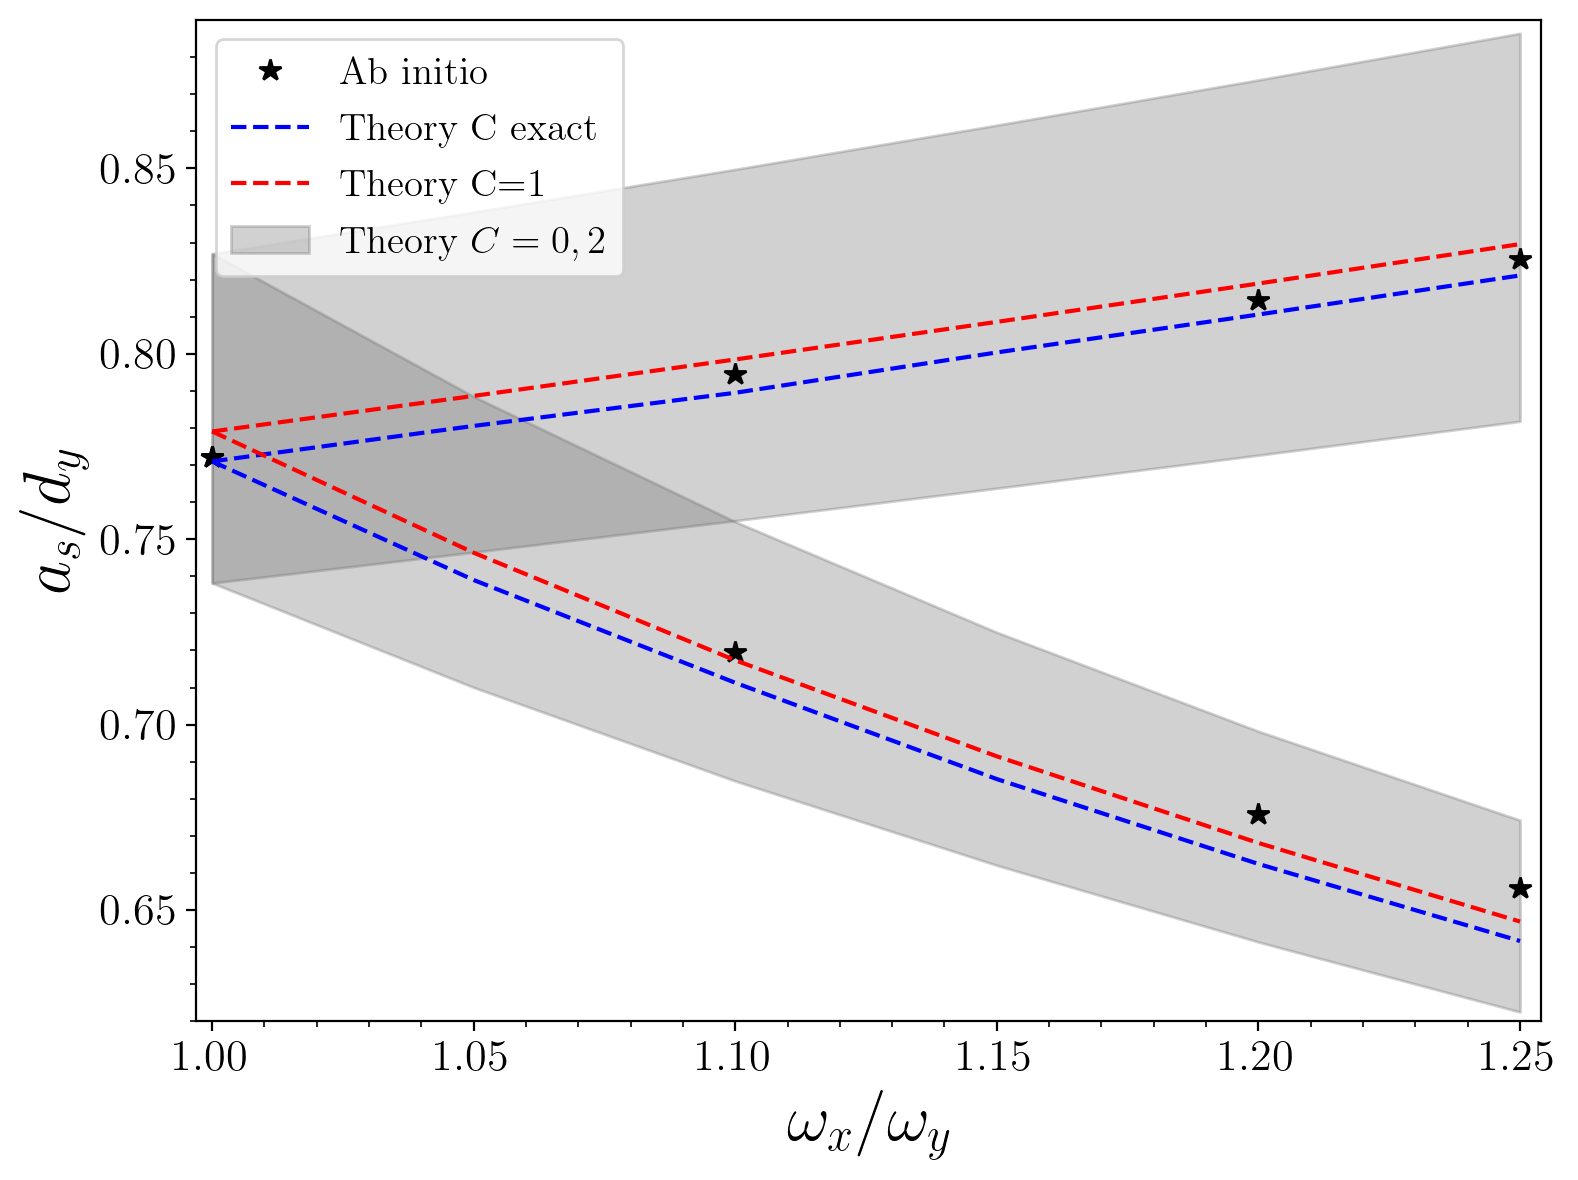
\includegraphics[width=0.5\textwidth]{/Users/tomy/PhD/Ultracold_Atoms_src/Analysis/q1d/Results/Figures/ICIR_q1D_Theory_band_coupling.png}
    	\caption{Same as Fig. \ref{fig:q3d ICIR} but in the quasi 1-D case with parameters: $V_y = 35.9E_R$, $\eta_z = 0.1$ and $\lambda=1000$ nm. }
    	\label{fig:q1D ICIR}
	\end{figure}
	
Results demonstrate that the assumption of $\mathcal{C}=1$ is not necessarily true for quasi 1-D and wrong for 3-D traps. The width of the shadow bands indicate that \textit{ab initio} calculations are essential to compare theory with experiments, until exact solutions including the anharmonicities are found.
%------------------------------------------------------------------------------------
\section{Origin of the asymmetric splitting of the ICIR} \label{sec:perturbation}
In this section we develop a perturbation theory to predict the position of an ICIR. As it will be shown, this perturbative scheme provides a simple explanation to the asymmetric splitting that is observed when the experimental setup becomes anisotropic by changing the longitudinal or the transversal frequencies. 

In order to follow a self-consistent approach the perturbed CM energies are used. The anharmonic terms of the trapping potential are then treated as a perturbation. $R^4$ and $R^6$ terms are expressed in terms of the Hermite Polynomials to make the integrals exactly solvable, yielding to
%\begin{widetext}
\begin{eqnarray}
E^{CM}_{\bfeq{n}} &=& \sum_{j=x,y,z} \hbar \omega_j(n_j + 1/2) \nonumber \\ 
&-& \frac{1}{1152V^2_j} \left[ 36V_j\hbar^2\omega^2_j(2n^2_j + 2n_j + 1) \right. \nonumber \\
&-&\left. \hbar^3 \omega^3_j (4n^3_j + 6n^2_j + 8n_j + 3)\right]
\label{eq:Perturbation CM E}
\end{eqnarray}

which is the first order perturbation term of the CM trapping potential, $n_j$ are the excitation levels in a given direction. Equation \eqref{eq:Perturbation CM E} give the energy of a single well. The inclusion of higher order correction terms render a triple well, and, as a consequence, can be used to describe multiwell effects. Notice that the perturbative scheme is only meaningful up to $2l+1$ order $\mathcal{O}(\hbar \omega_j)$, with $l = 0,1,2,...,$ as, otherwise, it yields unphysical results with negative energies, as they correspond to an unbounded potential associated with the Taylor expansion of the optical lattice. Consequently, the energy shift is given by:
\begin{eqnarray}
\epsilon &=& \mathcal{C} \eta_z - \sum_j \left[  \eta_j n_j - \eta^2_j \frac{\hbar \omega_y}{16V_j}n_j(n_j+1) \right. \nonumber \\
 &-&\left. \eta^3_j \left(\frac{\hbar \omega_y}{24V_j}\right)^2 n_j(4 + 3n_j + 2n^2_j)\right].
\label{eq:Perturbation shift}
\end{eqnarray}

Thus, we take as reference the isotropic setting, which has a frequency $\bar{\Omega}$ in all directions, then a change in the frequencies can be written as
\begin{eqnarray}
\omega_x &=& \bar{\Omega} + \Delta \omega_x, \\
\omega_y &=& \bar{\Omega} + \Delta \omega_y, \\
\omega_z &=& \bar{\Omega} + \Delta \omega_z.
\label{eq:perturbation variables}
\end{eqnarray}

Recall that any change in the frequencies will also affect the value of the characteristic length $d_y$, the $\eta_x$ and $\eta_z$ ratios, and the energy shift $\epsilon$, which then will become
\begin{eqnarray}
d_y &=& \bar{d_y} + \Delta d_y, \\
\eta_x &=& \bar{\eta_x} + \Delta \eta_x, \\
\eta_z &=& \bar{\eta_z} + \Delta \eta_z, \\
\epsilon &=& \bar{\epsilon} + \Delta \epsilon. 
\label{eq:perturbation variables 2 }
\end{eqnarray}

If we change the frequencies slightly all at once ($\Delta \omega_i \ll \omega_i $) the integral of Eq. \eqref{eq:ascE} can be Taylor expanded. Although we are interested in the case of changing only $\omega_x$. 

The result of the expansion is presented in terms of integrals of the form 
\begin{eqnarray}
&\mathcal{I}&(\epsilon, \eta_x, \eta_z, d_y, A, B) = \frac{1}{\sqrt{\pi}d_y} \nonumber \\
\int^\infty_0 &dt& \left( \frac{A\sqrt{\eta_x \eta_z} e^{\frac{\epsilon t}{2}}}{\sqrt{(1 - e^{-t}) (1 - e^{-\eta_x t}) (1 - e^{-\eta_z t})} } - Bt^{-\frac{3}{2}}\right). \nonumber \\
\label{eq:Integral perturbation}
\end{eqnarray}

Note that the scattering length corresponds with $\frac{1}{a_s} = - \mathcal{I}(\epsilon, \eta_x, \eta_z, d_y, 1, 1)$. Then after the expansion we have
\begin{eqnarray}
\frac{\bar{d_y}}{a_s} &=& - \mathcal{I}(\bar{\epsilon}, 1, 1, 1, 1, 1) \left( 1-\frac{\Delta d_y}{\bar{d_y}}\right) \nonumber \\
&-& \mathcal{I}\left(\bar{\epsilon}, 1, 1, 1, \frac{t}{2}, 0 \right) \Delta \epsilon \nonumber \\
&-&  \mathcal{I}\left(\bar{\epsilon}, 1, 1, 1, \frac{1 - e^{-t}(1+t)}{2(1-e^{-t})}, 0 \right) \Delta \eta_x \nonumber \\
&+& \mathcal{O}(\Delta \eta_x)^2 + \mathcal{O} (\Delta \epsilon)^2.
\label{eq:result perturbation}
\end{eqnarray}

We analyze up to first order in perturbation theory the imprint of a small change in the longitudinal frequency on the scattering length, and provide an explanation on the ICIR splitting, as schematically sketched in Fig. \ref{fig:ICIR scheme}. We study the influence of a change in the longitudinal frequency, $\omega_x$. The unique ICIR located at point A (cyan circle) for the isotropic setting will bifurcate into two different branches (cyan arrows). Notice that while the top branch increases abruptly, the bottom one is only slightly affected by the frequency change.

\begin{figure}[htbp!]
\centering
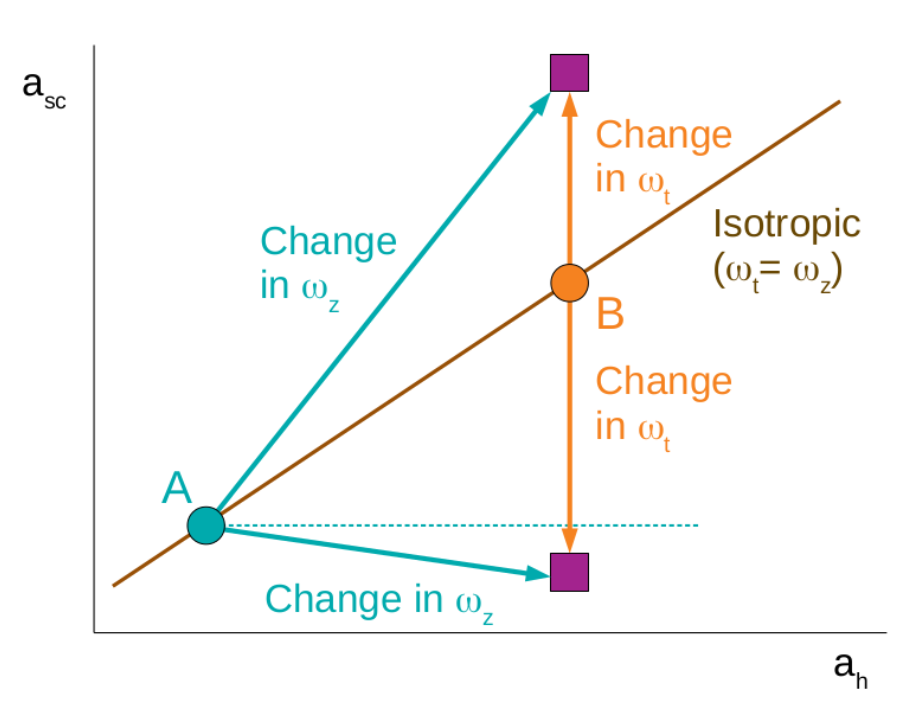
\includegraphics[width=0.5\textwidth]{ICIR_scheme_Perturb}
\caption{The inelastic confinement-induced resonances for the isotropic setting (brown line) bifurcate in two different branches when the traps becomes anisotropic. In point A (cyan circle), the longitudinal frequency ($\omega_x$) is decreased, and then the two cyan branches separate rightwards, moving one of them upwards, while the other one remains almost constant. In point B (orange circle), the transversal frequencies ($\omega_y = \omega_z$) are increased, and then the two vertical orange branches separate one moving upwards and the other one downwards.}
\label{fig:ICIR scheme}
\end{figure}

Changing only the longitudinal frequency implies $\Delta d_y = 0$ since it remains constant. As in the experiment, we assume $\Delta \omega_x < 0$. Then
\begin{eqnarray}
\Delta \eta_x = \frac{\Delta \omega_x}{\bar{\Omega}},
\label{eq:Delta eta_x perturbed}
\end{eqnarray}

which renders a negative contribution to the scattering length that tends to decrease ($a_s < \bar{a_s}$). Regarding the correction of the energy shift, the interpretation is more involved since it depends on the excitation level. The main contribution is
\begin{eqnarray}
\Delta \epsilon \cong (n_x - \mathcal{C}) \frac{|\Delta \omega_x|}{\bar{\Omega}},
\label{eq:Delta shift perturbed}
\end{eqnarray}

which is positive for $n_x > C$ and negative for $n_x=0$. 

Let us now discuss the different behavior of the ICIR's depending on whether they have excitations in the longitudinal direction, $x$, or not. On the one hand, when the ICIR has no CM excitations in the $x$ direction, then the last two terms appearing in Eq. \ref{eq:result perturbation} will be negative, and, as a consequence, the value of the scattering length will be smaller than in the isotropic setting. Contrary, if the ICIR has some CM excitations in the $x$ direction, the new scattering length will increase with the value of $n_x$, as the second term in Eq. \ref{eq:result perturbation} will be positive and dominates over the second one; Moreover, the increment in the scattering length will increase with the number of excitations in the $x$ direction, $n_x$, and, as a consequence, the ICIR splitting will become more asymmetric.

Finally, Eq. \ref{eq:Delta shift perturbed} can be used to explain the extreme asymmetry between the shadow bands in the 3-D case. In Fig. \ref{fig:q3d ICIR} the prediction obtained with the exact $\mathcal{C}$ is in better agreement to $\mathcal{C}=0$ than $2$. Substituting in the last expression for the energy shift $n_x = 4$ gives $\Delta \epsilon(\mathcal{C}=0) = 4\frac{|\Delta \omega_x|}{\bar{\Omega}}$ and $\Delta \epsilon(\mathcal{C}=2) = 2\frac{|\Delta \omega_x|}{\bar{\Omega}}$. The exact value of the parameter is $0.52 \pm 0.03$, which corresponds with $\Delta \epsilon(\mathcal{C}=0.52) = 3.48\frac{|\Delta \omega_x|}{\bar{\Omega}}$. As presented in Eq. \eqref{eq:ascE}, the scattering length, $a_s$ have an exponential dependence on the energy shift, as a consequence the asymmetry between both predictions is exponentially increased.
%Comentario de que en el 200 las bandas se van haciendo más estrechas y en el 020 más anchas o algo así

%------------------------------------------------------------------------------------
\section{Conclusions}
Inelastic Confinement-Induced Resonances has shown to be a fundamental natural process since they appear in any trapped anharmonic-quantum system where the CM and relative coordinates present a non-vanishing coupling. In this work we expand the existing studies on ICIR's in order to shed light to some theoretical unsolved questions. 

As mentioned, in \cite{PhysRevLett.109.073201} the authors presented a satisfactory agreement between their theoretical model (CRC) and the resonance measurements of \cite{PhysRevLett.104.153203}. Here, we generalize the CRC model by introducing the $\mathcal{C}$ parameter which was assumed to be exactly $1$. Our generalization has found an explanation of why the previous assumption works for quasi 1-D  but not for 3-D confinements. We first show the results for 3-D from which we conclude that \abinitio calculations are needed to obtain good theoretical predictions when giving the ICIR position, without this input $\mathcal{C}=1$ prediction obtain considerably large mean absolute errors. This is not the case for quasi 1-D confinements where the theory predictions are much more insensitive on the value of $\mathcal{C}$ since its dependence is modulated by the anisotropy $\eta_z$. 

Furthermore, the reason that makes the value of the parameter decrease from $0.82 \pm 0.01$ (quasi 1-D) to $0.52 \pm 0.03$ (3-D) is associated with the level mixing. In harmonic confinements the diabatic states cross at $\mathcal{C}=1$, but when anharmonic terms are included the pure states couple to each other forming mixed states. Moreover, the greater the anisotropy is the closer in energies are one states to others and, therefore, stronger the mixing is. Collectively, our results on both confinement dimensions provide evidence for that.

Another important finding in the understanding of the ICIR's is the origin of their asymmetric splitting for non-zero anisotropies. Here, we have develop a perturbative scheme to account for small variations around the isotropic setting. Equation \eqref{eq:ascE} is Taylor expanded in terms of the characteristic trap length $d_y$, the energy shift $\epsilon$ and the anisotropy in the $x$ direction $\eta_x$ to first order. The appearance of the asymmetric splitting is qualitatively explained with the help of Eq. \eqref{eq:Delta shift perturbed}.

Future research on ultracold atoms scattering in mixed dimensions might extend the explanations given in this study of the nature of ICIR's. Recently, an experiment presented in \cite{PhysRevLett.104.153202} detect loosing mechanisms in a mixture of ultracold 3D(Rb)-2D(K) gases. This system is coupled not only by the anharmonicities of the optical trap, by also by the heterogeneous combination of atomic species. This motivates to continue investigating the ICIR's being a good starting point to test the \abinitio and theoretical approaches shown in this paper.
%------------------------------------------------------------------------------------
\section{Anknowledgements}
movidas
%------------------------------------------------------------------------------------

\bibliographystyle{unsrtnat}
\bibliography{q1d_q3d_perturbationCitation.bib}

\end{document}

















